
\documentclass[11pt]{article}


% Document config
\setlength{\parindent}{12pt}
\usepackage[letterpaper, margin=1in]{geometry}
\usepackage[spanish]{babel}
\usepackage[utf8]{inputenc}
\usepackage{tikz}
\usepackage{hyperref}
\usepackage{color}
\usepackage{xcolor}
\usepackage{float}
\usepackage{tcolorbox}
\usepackage[nottoc]{tocbibind}
\usepackage{graphicx}
\usepackage{listings}
\usepackage{lineno}
\usepackage{fancyvrb}
\usepackage[utf8]{inputenc}
\graphicspath{ {./Documents/Tarea2/} }

\bibliographystyle{plain}

% Color definitions
\definecolor{darkblue}{rgb}{0 , 0.054 , 0.196}
\definecolor{mygreen}{rgb}{0,0.6,0}
\definecolor{mygray}{rgb}{0.8,0.8,0.8}
\definecolor{codeBG}{rgb}{0.9, 0.97, 0.9}
\definecolor{mymauve}{rgb}{0.58,0,0.82}


\definecolor{codegreen}{rgb}{0,0.6,0}
\definecolor{codegray}{rgb}{0.5,0.5,0.5}
\definecolor{codepurple}{rgb}{0.58,0,0.82}
\definecolor{backcolour}{rgb}{0.95,0.95,0.92}
 
\lstdefinestyle{miestilo}{
    backgroundcolor=\color{backcolour},   
    commentstyle=\color{codegreen},
    keywordstyle=\color{red},
    numberstyle=\tiny\color{codegray},
    stringstyle=\color{black},
    basicstyle=\footnotesize,
    breakatwhitespace=false,         
    breaklines=true,                 
    captionpos=b,                    
    keepspaces=true,                 
    numbers=left,                    
    numbersep=5pt,                  
    showspaces=false,                
    showstringspaces=false, 
    showtabs=false,                  
    tabsize=2
}
 
\lstset{style=miestilo}


%\addto\captionsspanish{% Replace "english" with the language you %use
%  \renewcommand{\contentsname}%
%    {Tabla de contenidos}%
%}



%\title{
%{
%    \begin{tikzpicture}[overlay, remember picture]
%        \node[anchor=north west, %anchor is upper left corner of %the graphic
%            xshift=3cm, %shifting around
%            yshift=-4cm] 
%            at (current page.north west) %left upper corner of the %page
%        {
\includegraphics[height=1.3cm]{logoEIE.png}}; 
%    \end{tikzpicture}
%    \begin{tikzpicture}[overlay, remember picture]
%        \node[anchor=north east, %anchor is upper left corner of %the graphic
%            xshift=-3cm, %shifting around
%            yshift=-4cm] 
%            at (current page.north east) %left upper corner of the %page
%        {
\includegraphics[height=1.3cm]{logoUCR.png}}; 
%    \end{tikzpicture}
%    \Large 
%        \textbf{Universidad de Costa Rica}\\
%        Facultad de Ingeniería\\
%        Escuela de Ingeniería Eléctrica\\~\\
%        \texttt{IE-0313} Electronica I
%    }
%    ~\\~\\
%    {\LARGE Demostración del JFET}
%}
%\author{Dennis Chavarría Soto B82097\\}
%\date{II ciclo\\25 de octubre de 2019}%


\documentclass[12pt]{article}

\usepackage{graphicx}
\usepackage[letterpaper, margin=1in]{geometry}
\usepackage{times}
\renewcommand{\familydefault}{\sfdefault}
\usepackage[spanish]{babel}
\usepackage[utf8]{inputenc}
\usepackage{float}%para acomodar imagenes
\usepackage{hyperref}%agrega hipervinculos a el indice y citas
\usepackage{url}%citar paginas web
\usepackage{apacite}%estilo apa
\usepackage{minted} % para resaltar código fuente
%\usepackage{listings}%para insertar el codigo en 
%\usepackage{moreverb} 

\usepackage[none]{hyphenat}%justifica el texto sin dividir palabras





\begin{document}
\sloppy%para que justifique el texto correctamente

\newmintedfile[mycplusplus]{c++}{
    linenos, % muestra el número de línea
    numbersep=5pt, % separación entre el código y el número de línea
    gobble=0, % columna desde la que empieza a mostrar código
    frame=lines, % dibuja las líneas enmarcando el código
    framesep=2mm, % separación entre la línea y el código
    tabsize=3, % tamaño de la tabulación
}

\newmintedfile[mypython]{py}{
    linenos, % muestra el número de línea
    numbersep=5pt, % separación entre el código y el número de línea
    gobble=0, % columna desde la que empieza a mostrar código
    frame=lines, % dibuja las líneas enmarcando el código
    framesep=2mm, % separación entre la línea y el código
    tabsize=3, % tamaño de la tabulación
}
\renewcommand{\refname}{}

\bibliographystyle{apacite}%estilo apa
\nocite{*} % si quieren que todas las referencias de su bibtex aparezcan en el documento

\begin{titlepage}
		\bf
		\centering
		
\includegraphics[width=0.20\textwidth]{logoEIE.png}			
		\hspace{7cm} 
		
\includegraphics[width=0.30\textwidth]{logoUCR.png}	
		\par
		\vspace{2cm}			
		{\scshape\large Universidad de Costa Rica \par}
		\vspace{0.6cm}
		{\scshape\large Facultad de Ingenieria\par}
		\vspace{0.6cm}
		{\scshape\large Escuela de Ingenieria Eléctrica\par}
		\vspace{0.6cm}
		{\scshape\large Estructuras Abstractas De Datos y Algoritmos Para Ingeniería   \par}
		\vspace{1.5cm}		
		{\scshape\large Laboratorio 5: Stack-Queue y Árboles BST\par}
		\vspace{2.5cm}		
		{\scshape\large Estudiantes:\\ Dennis Chavarría Soto (B82097)  \par}
		\vspace{2.5cm}		
		{\scshape\large Profesor:\\ Ricardo Román Brenes; M. Sc. \par}
		\vspace{2.5cm}
		{\scshape\large II ciclo 2019 \par}
\end{titlepage}



%\begin{document}
%\maketitle 
\tableofcontents
\listoffigures
\newpage

\hrule
\hrule

\newpage
\section{Solución}

La premisa fundamental al resolver los problemas propuestos fue, no cambiar los demás archivos que no fueran el Main.cpp que invoca toda la lógica del programa, así pues, por cada enunciado relacionado con la implementación de código, se referirá principalmente a los main.

\subsection{Dada una hilera de caracteres que contenga pares de parentesis, corchetes o boquillas, con letras, sea
capaz de decir si dicha hilera esta bien escrita en el sentido de los pares de par ´ entesis; o sea, ´
que siempre que se abra un parentesis, se cierre antes de cerrar uno de otro tipo}

Para el primer programa se instancia un stack y, luego, establecen, al inicio, tres identificadores. El programa cuenta con un condicional para determinar si la cadena ingresada está vacía, en dado caso, se termina el programa y no se ejecuta lógica alguna.

Si la cadena ingresada cumple con lo esperado, los identificadores se establecen como 0 apenas ingresan a un ciclo for que depende de la cantidad de argumentos ingresados (La cantidad de hileras), esto es necesario para pasar por cada hilera que el usuario ingresa, luego otro ciclo, de tipo for, se utiliza para recorrer cada hilera comparando si los elementos son aperturas de paréntesis, corchetes o boquillas, en dado caso aumenta el valor de id2, que corresponde a la cantidad de aperturas, luego compara si se encuentra un elemento de cerrado, y aumenta id3, que indica esta cantidad de terminos. Después de estos condicionales, hay uno tercero; al detectar un elemento de cerrado, compara si su homólogo de apertura está guardado en la última posición del stack, si esto es así, aumenta el valor de id. Si al terminar todos los recorridos, los id´s no son iguales, se concluye que la hiler es inválida. Esto se consigue con el condicional que está al final del método main.

Es importante destacar, cuando se está recorriendo por los términos de las hileras y se revisa el último elemento del stack, esto se consigue gracias a que, en el archivo Stack.h se encuentran diferentes métodos, entre ellos el de peek y el de pop; el primero permite revisar el último elemento de la pila, si coincide con el homólogo de cerrado que se encuentra en la hilera, gracias al recorrido que logra el ciclo for se usa el método del stack llamado pop, el cuál elimina el elemento más reciente agregado. De esta forma, apenas se abre un paréntesis, se esperaría que este sea el primer en ser cerrado, de forma que los más viejos son los últimos. Tal lógica se implementó y permitió el funcionamiento del código.

El resultado que se consigue es el deseado, el usuario introduce las hileras con los paréntesis, por ejemplo, y si no se tiene el respectivo elemento de cerrado, se indica \textit{cuál cola entre las proporcionadas} es la incorrecta.

El archivo main depende de Element.h y Stack.h, que definen alguno métodos para la obtención de valores y formato, en el caso del primero; para el segundo, se define la clase que consta de todos los métodos para agregar, borrar o visualizar elementos en el stack.


\newpage
\subsection{Dada una cantidad de colas y una proporcion de prioridad, construir un sistema de colas de ´
prioridad, donde de manera aleatoria, se agreguen elementos a las colas y basada con la proporcion de prioridades, se eliminen los elementos del sistema.}

La solución para este problema se consiguió con el código contenido en el archivo a.cpp; para ellos se requiere de bibliotecas como Chrono y Random, así como las cabeceras Queue.h y Element.h; este programa tiene un método que permite obtener números aleatorios.

En el método main se encuentra toda la lógica del programa y, por medio de variables como elements, rand-num, num-cola y nuevo-elemento, se consigue guardar la cantidad de colas que el usuario desea, luego, la cantidad de items que las colas almacenarán. Entre lo primero se instancia un arreglo de colas, pues, se desea que sea dinámico. El programa debe asignar la cantidad de elementos que guardará cada cola como 0, al inicio; luego, con ayuda de un ciclo for, se añaden elementos en colas aleatorias, estos también lo son y cada numero pseudoaleatorio generado se obtiene gracias al método mencionado inicialmente. Sin embargo, al asignar los elementos, se tienen dos condicionales, para garantizar, al máximo posible, que todas las colas tengan al menos un elemento; es decir, si el numero de cola generado aleatoriamente lleva a que una de ellas sea discriminada y no guarde elementos, estos detectores le asingarán el id de cola, para que le almacenen datos. Después de todo esto, se guardan.

El procedimiento de almacenamiento de datos en cada cola es complicado y susceptible a fallas, por ello, se incluye un ciclo que imprime al usuario los datos que componen las colas. Seguido a tal muestreo, se definen las variables k, p, elemento, prioridad y posición, estas se utilizan en un ciclo para determinar en cuál cola se encuentra, la máxima cantidad de elementos que puede eliminar de ella según la proporción de prioridad establecida. En tal ciclo, hay un primer condicional que realiza lo anteriormente mencionado, luego se aumenta un contador para saber cuando se alcanza el tope por prioridad y otro condicional verifica esta condición; este último tiene otro, el cuál identifica si ya se alcanzó el máximo de prioridad; osea, cuando se debe empezar otra vez con la primera relación de proporción que introduce el usuario. El valor de k tiene la función de que, se utiliza para navegar a través de los valores que definen esta proporción; la variable p indica la cola en la que se encuentra.

Al ejecutar toda la lógica anterior, el resultado es que, el usuario introduce la cantidad de colas, el programa define una cantidad máxima de 17 elementos que serán los que se almacenarán en la cola, luego, a partir de la prioridad (3:2:1 por ejemplo) indicada, se empiezan a eliminar los elementos contenidos y se muestran en la pantalla. 

Este programa también incluye el archivo element.h con los mismos métodos que el stack, así como el Queue.h que define los métodos para agregar y eliminar elementos. Como consideración importante, la cola introduce los valores y usa el orden FIFO, el primero agregado es el primero que se elimina, contrario al stack. 


\newpage
\subsection{Utilizando el modelo de arbol de búsqueda binaria realice las siguientes operaciones en orden: ´
a) creacion del árbol ´
b) inserciones: 4, 7, 2, 9, 5, 6, 1, 0, 15, 3
c) borrados: 2, 6, 0, 15
d) balanceo}

En las siguientes figuras se encuentra la descripción del procedimiento que se debe tomar para cumplir con los requisitos del problema, sin embargo, para complementar, se destaca que para el inciso a, se debe instanciar o crear un árbol que tendrá un primer elemento, la raíz, tal y como se explica, sin embargo, esta apuntará a las primeras ramas, que serán el hijo mayor y el menor, a partir de aquí se debe considerar para el inciso b que, los hijos menores al valor de la raíz (el 4) siempre van a la izquierda, y, siempre, los hijos mayores al valor agregado a la izquierda, inmediatamente después de la raíz, van a la derecha; a la izquierda de este irán los menores; lo mismo ocurre con el lado derecho, los hijos del nodo con valor igual a 7. Esta relación debe mantenerse entre todos los descendientes.

Al borrar los elementos, para el inciso b, se tiene que, el puntero que indicaba la dirección de memoria del nodo eliminado, debe cambiar. Al hacer el diagrama se consigue borrando lo que se desea, pero una implementación computacional implica que el puntero, o la dirección de siguiente elemento, indique un nuevo nodo, para ello, como se explica en las siguientes figuras, se debe elegir entre el nodo que contiene el mayor valor que se encuentre en la raíz izquierda, sino, se elige el menor a la derecha y al que se elige, se apunta con el puntero del hijo borrado para el nodo inmediatamente anterior. 

Considérese que los signos de pregunta en la parte c, indican que ahí se ha borrado un nodo, para el caso de la rama izquierda, se ve que hay una flecha que ahora apunta al nodo con el valor 3, pues, ese será el que rebalanceará tal rama. Entonces el árbol c indica

\newpage
\begin{figure}[H]
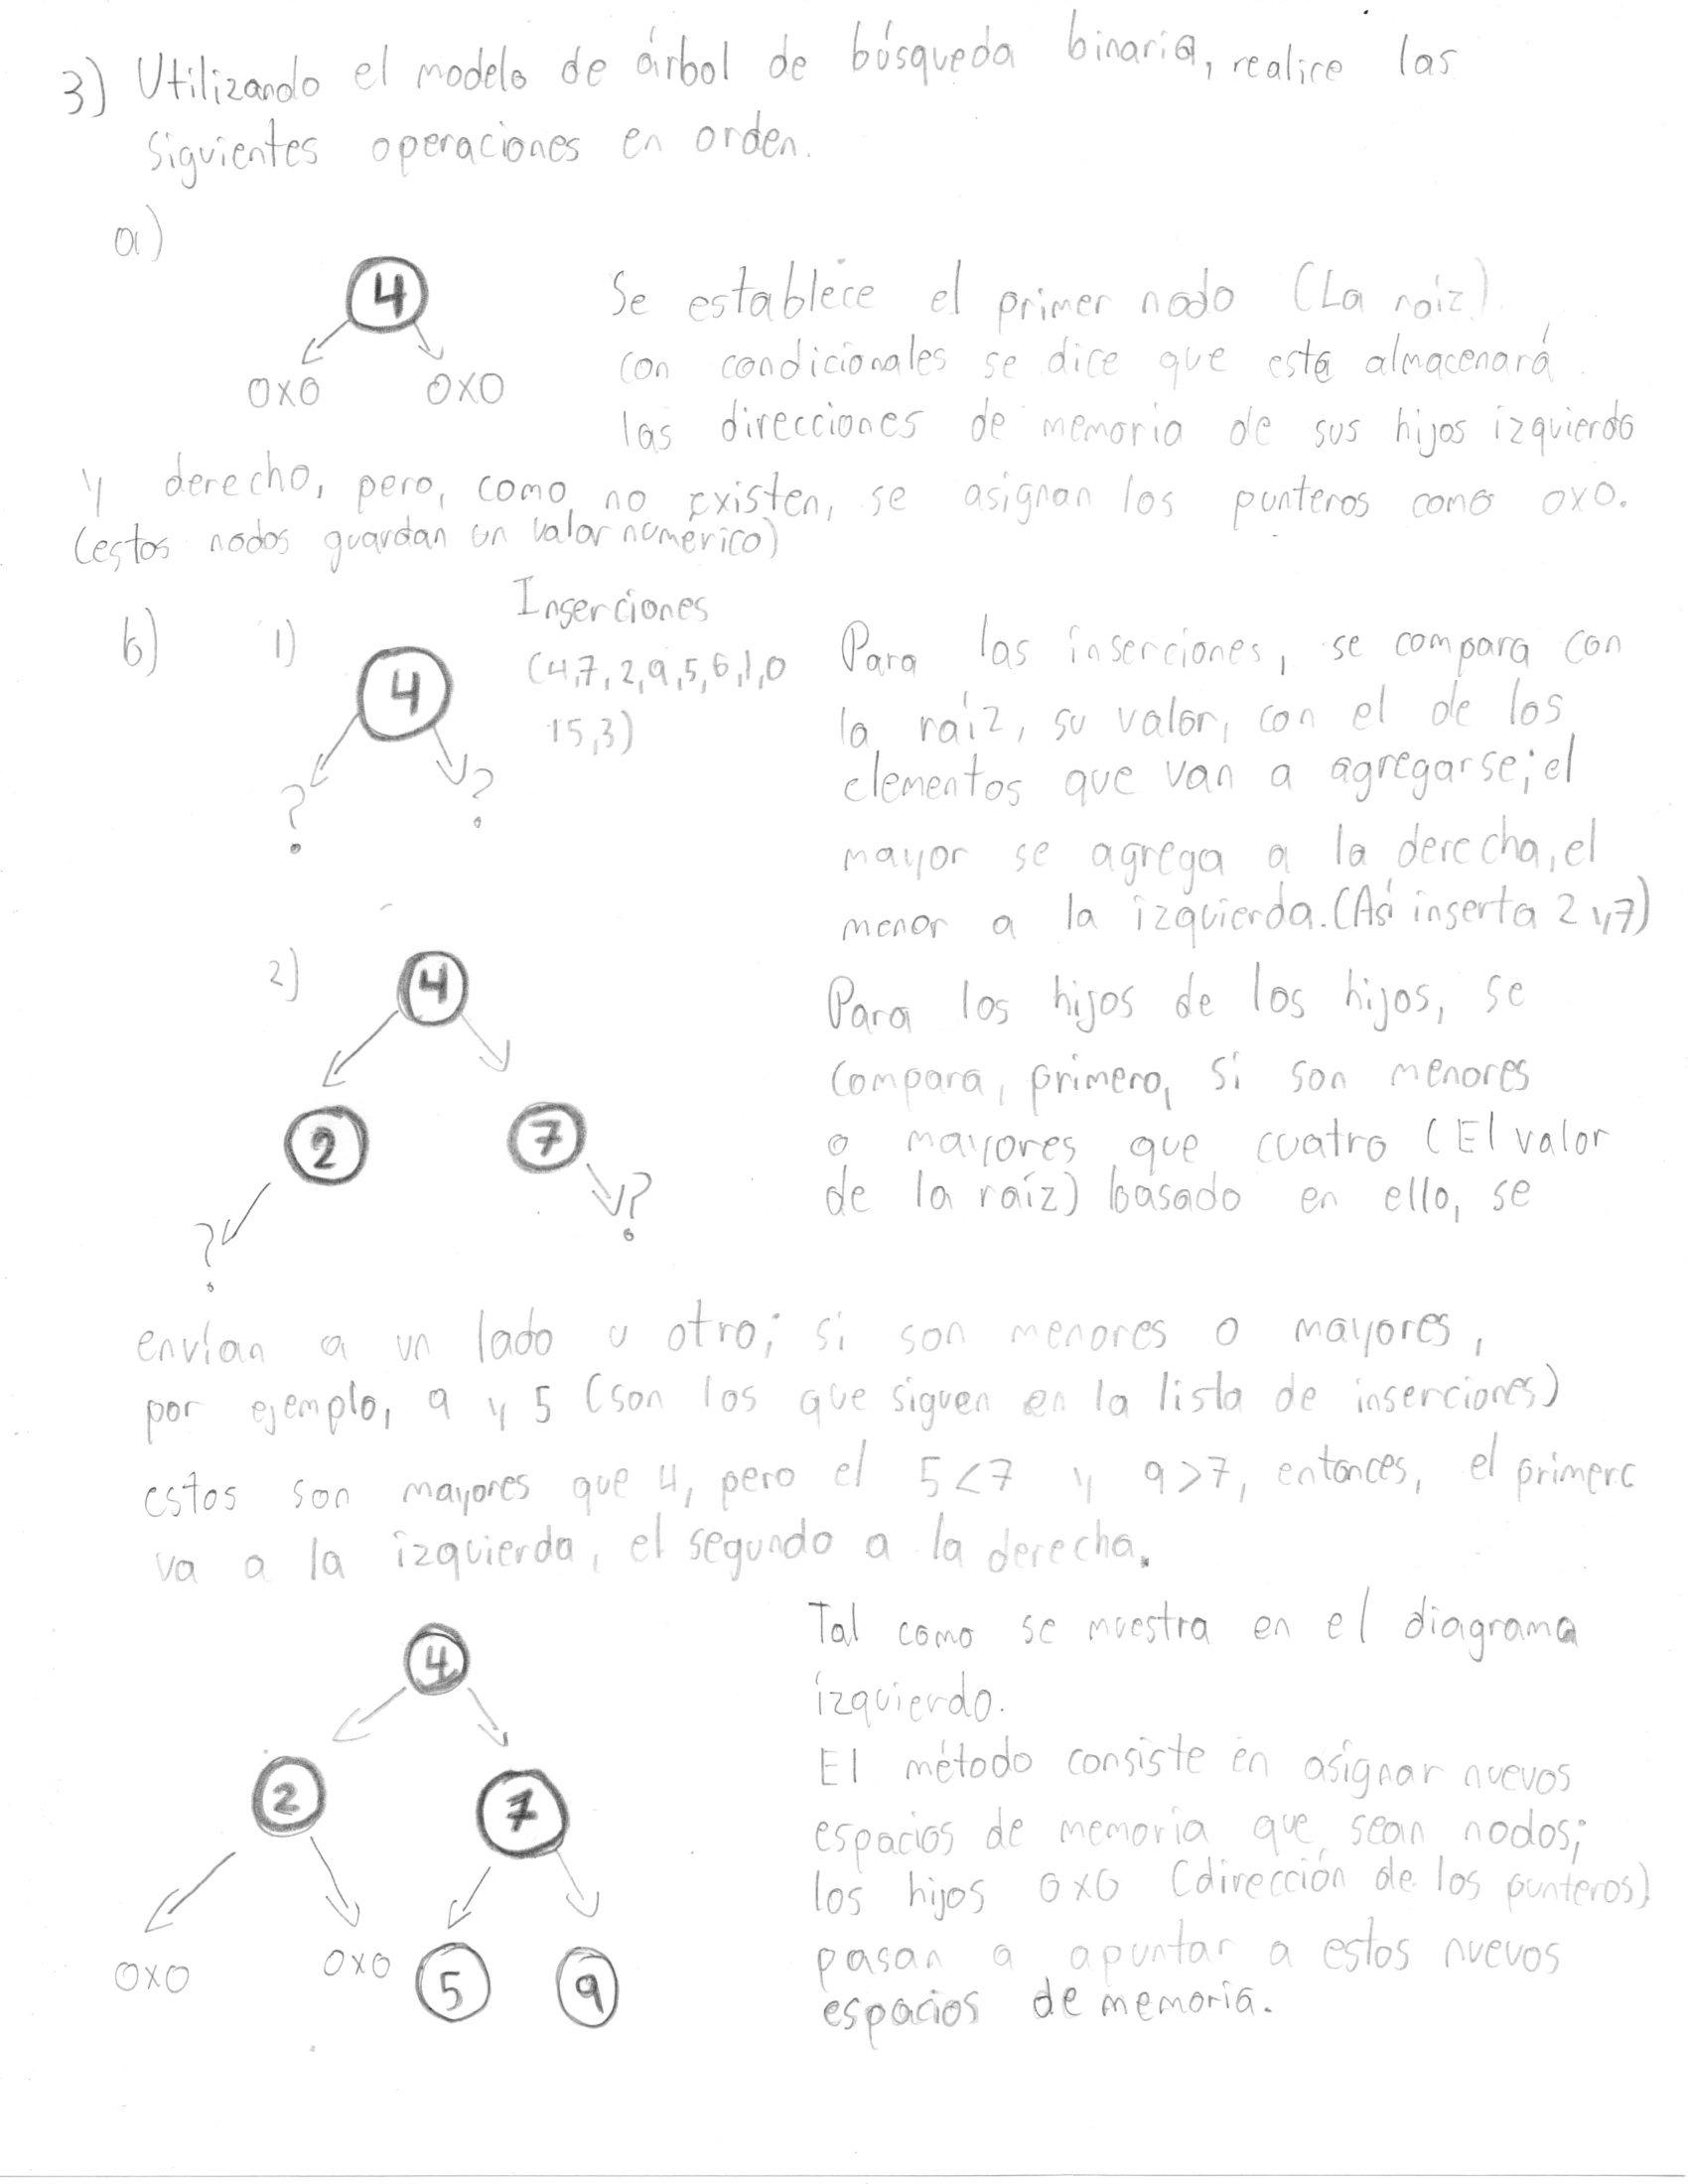
\includegraphics[width=18.5cm]{foto1.jpg}
\centering
\end{figure}

\newpage
\begin{figure}[H]
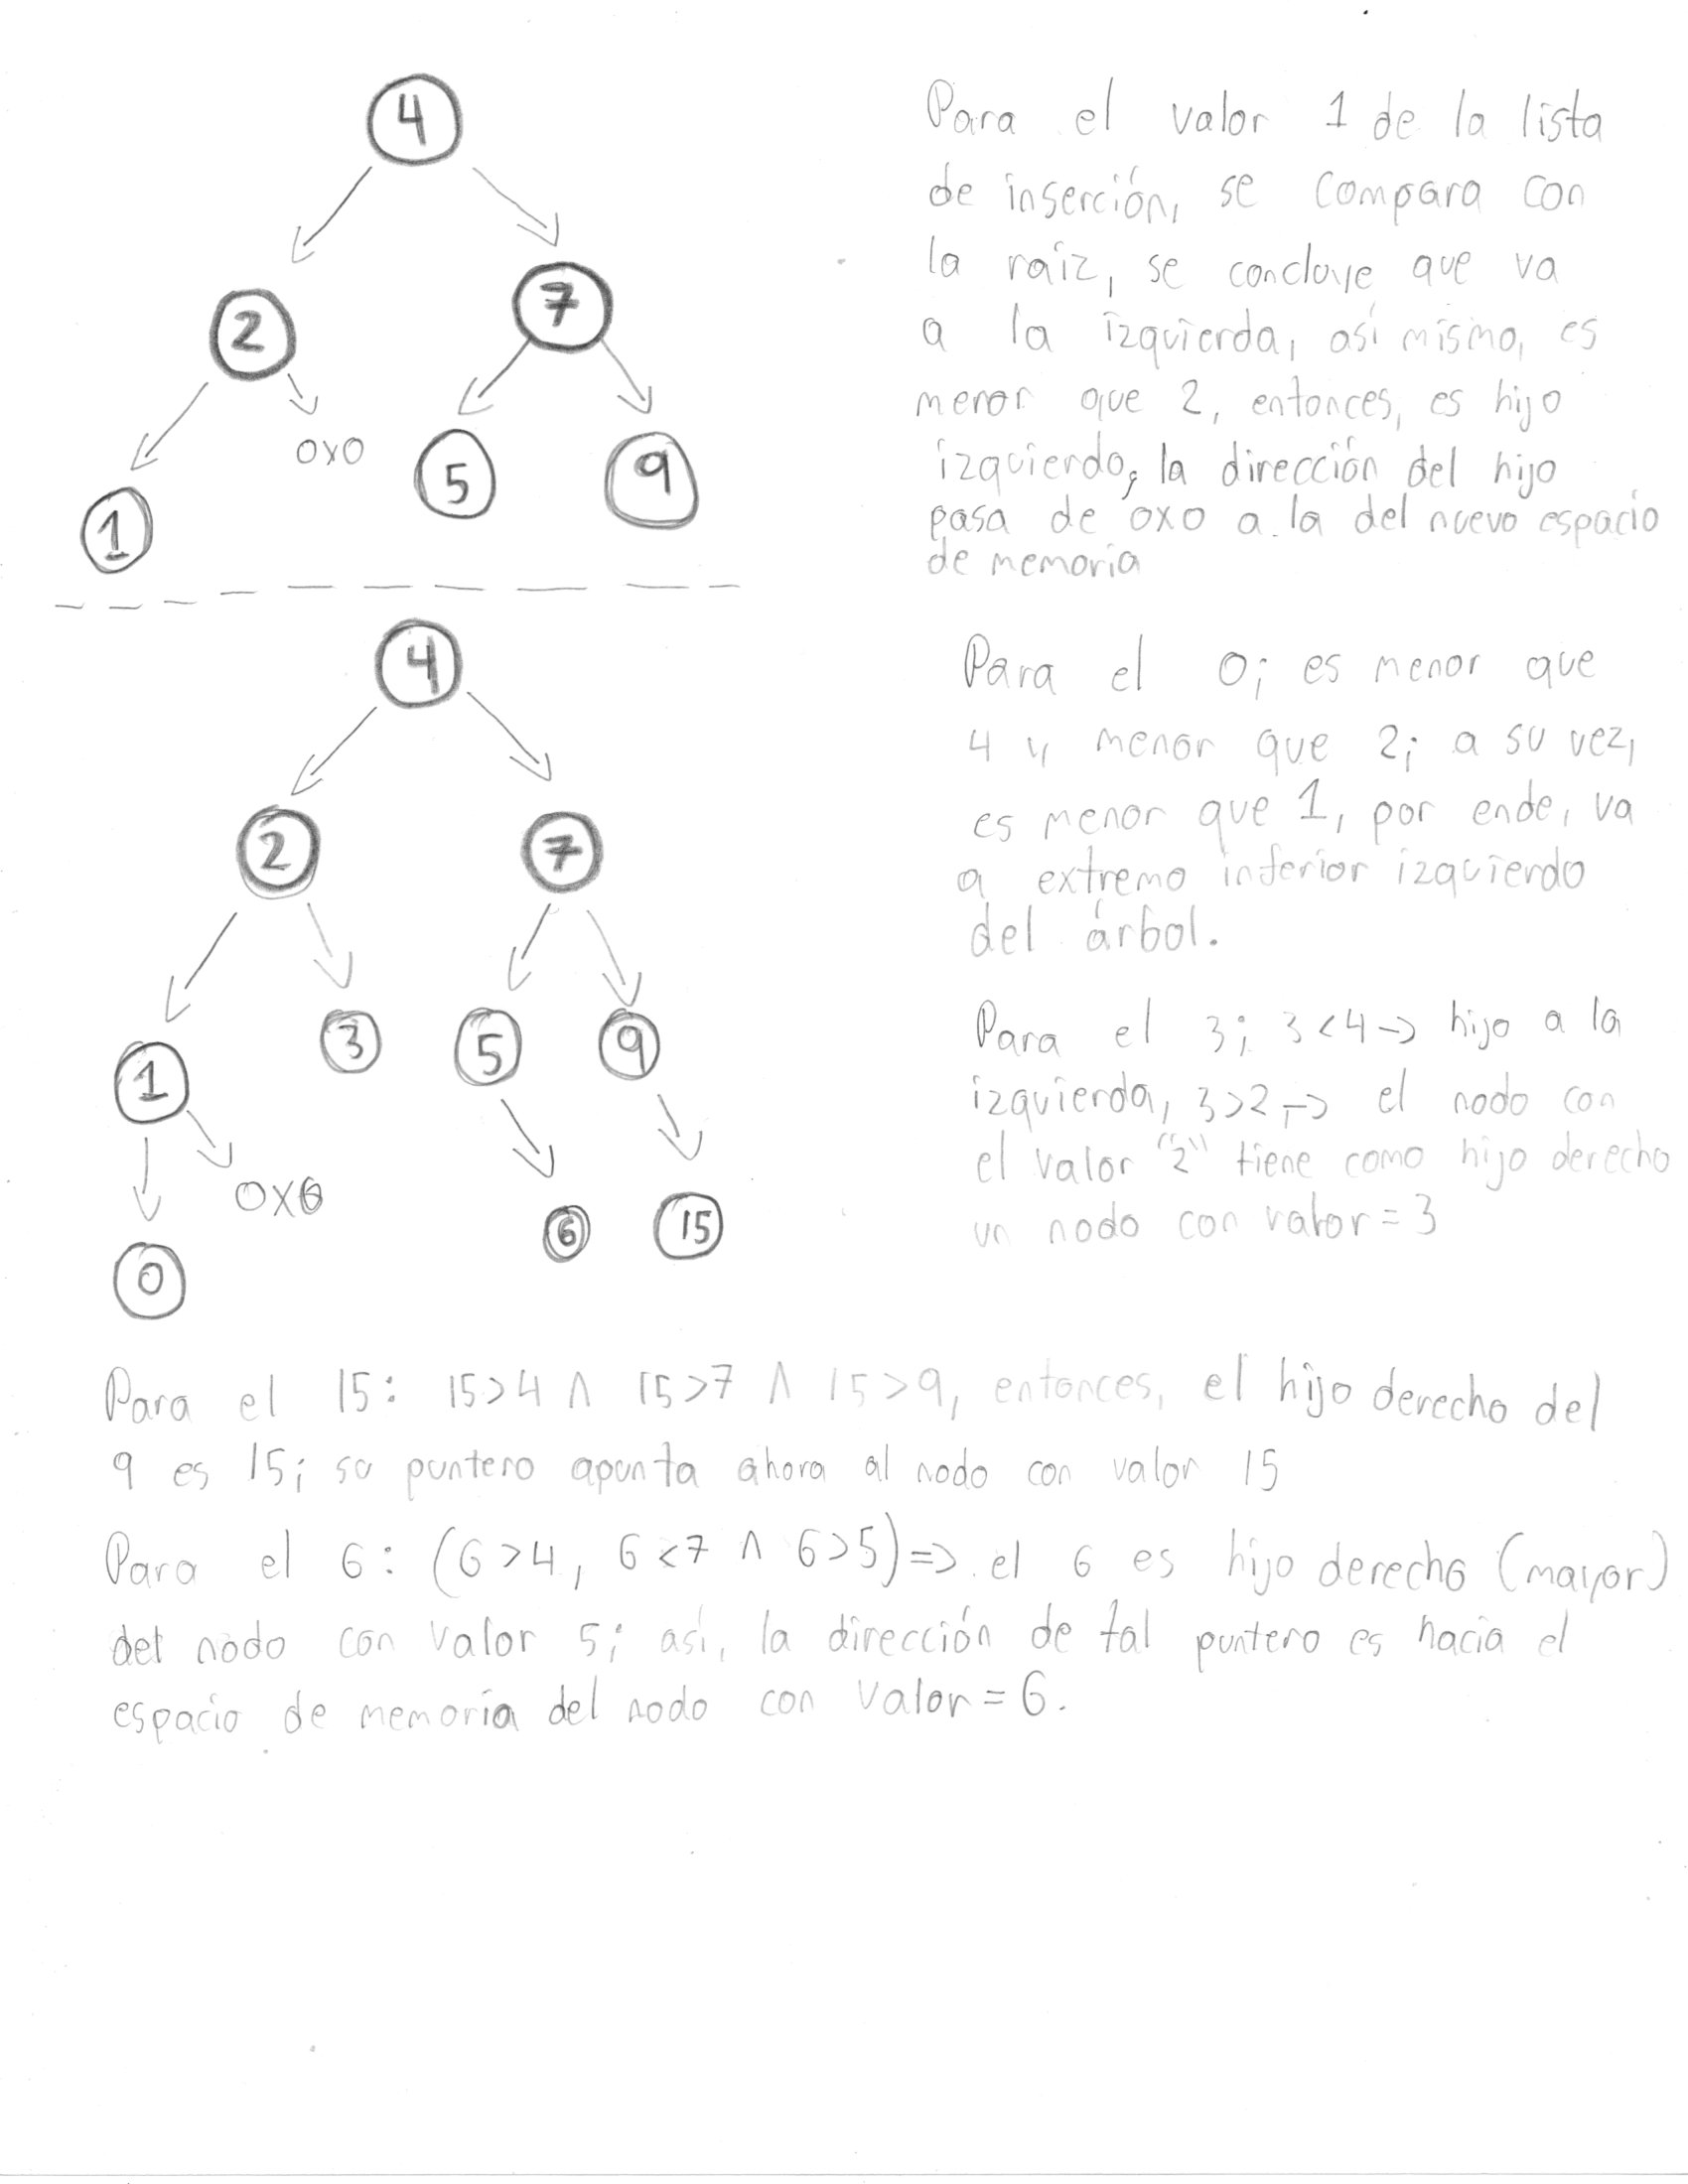
\includegraphics[width=18.5cm]{foto2.jpg}
\centering
\end{figure}

\newpage
\begin{figure}[H]
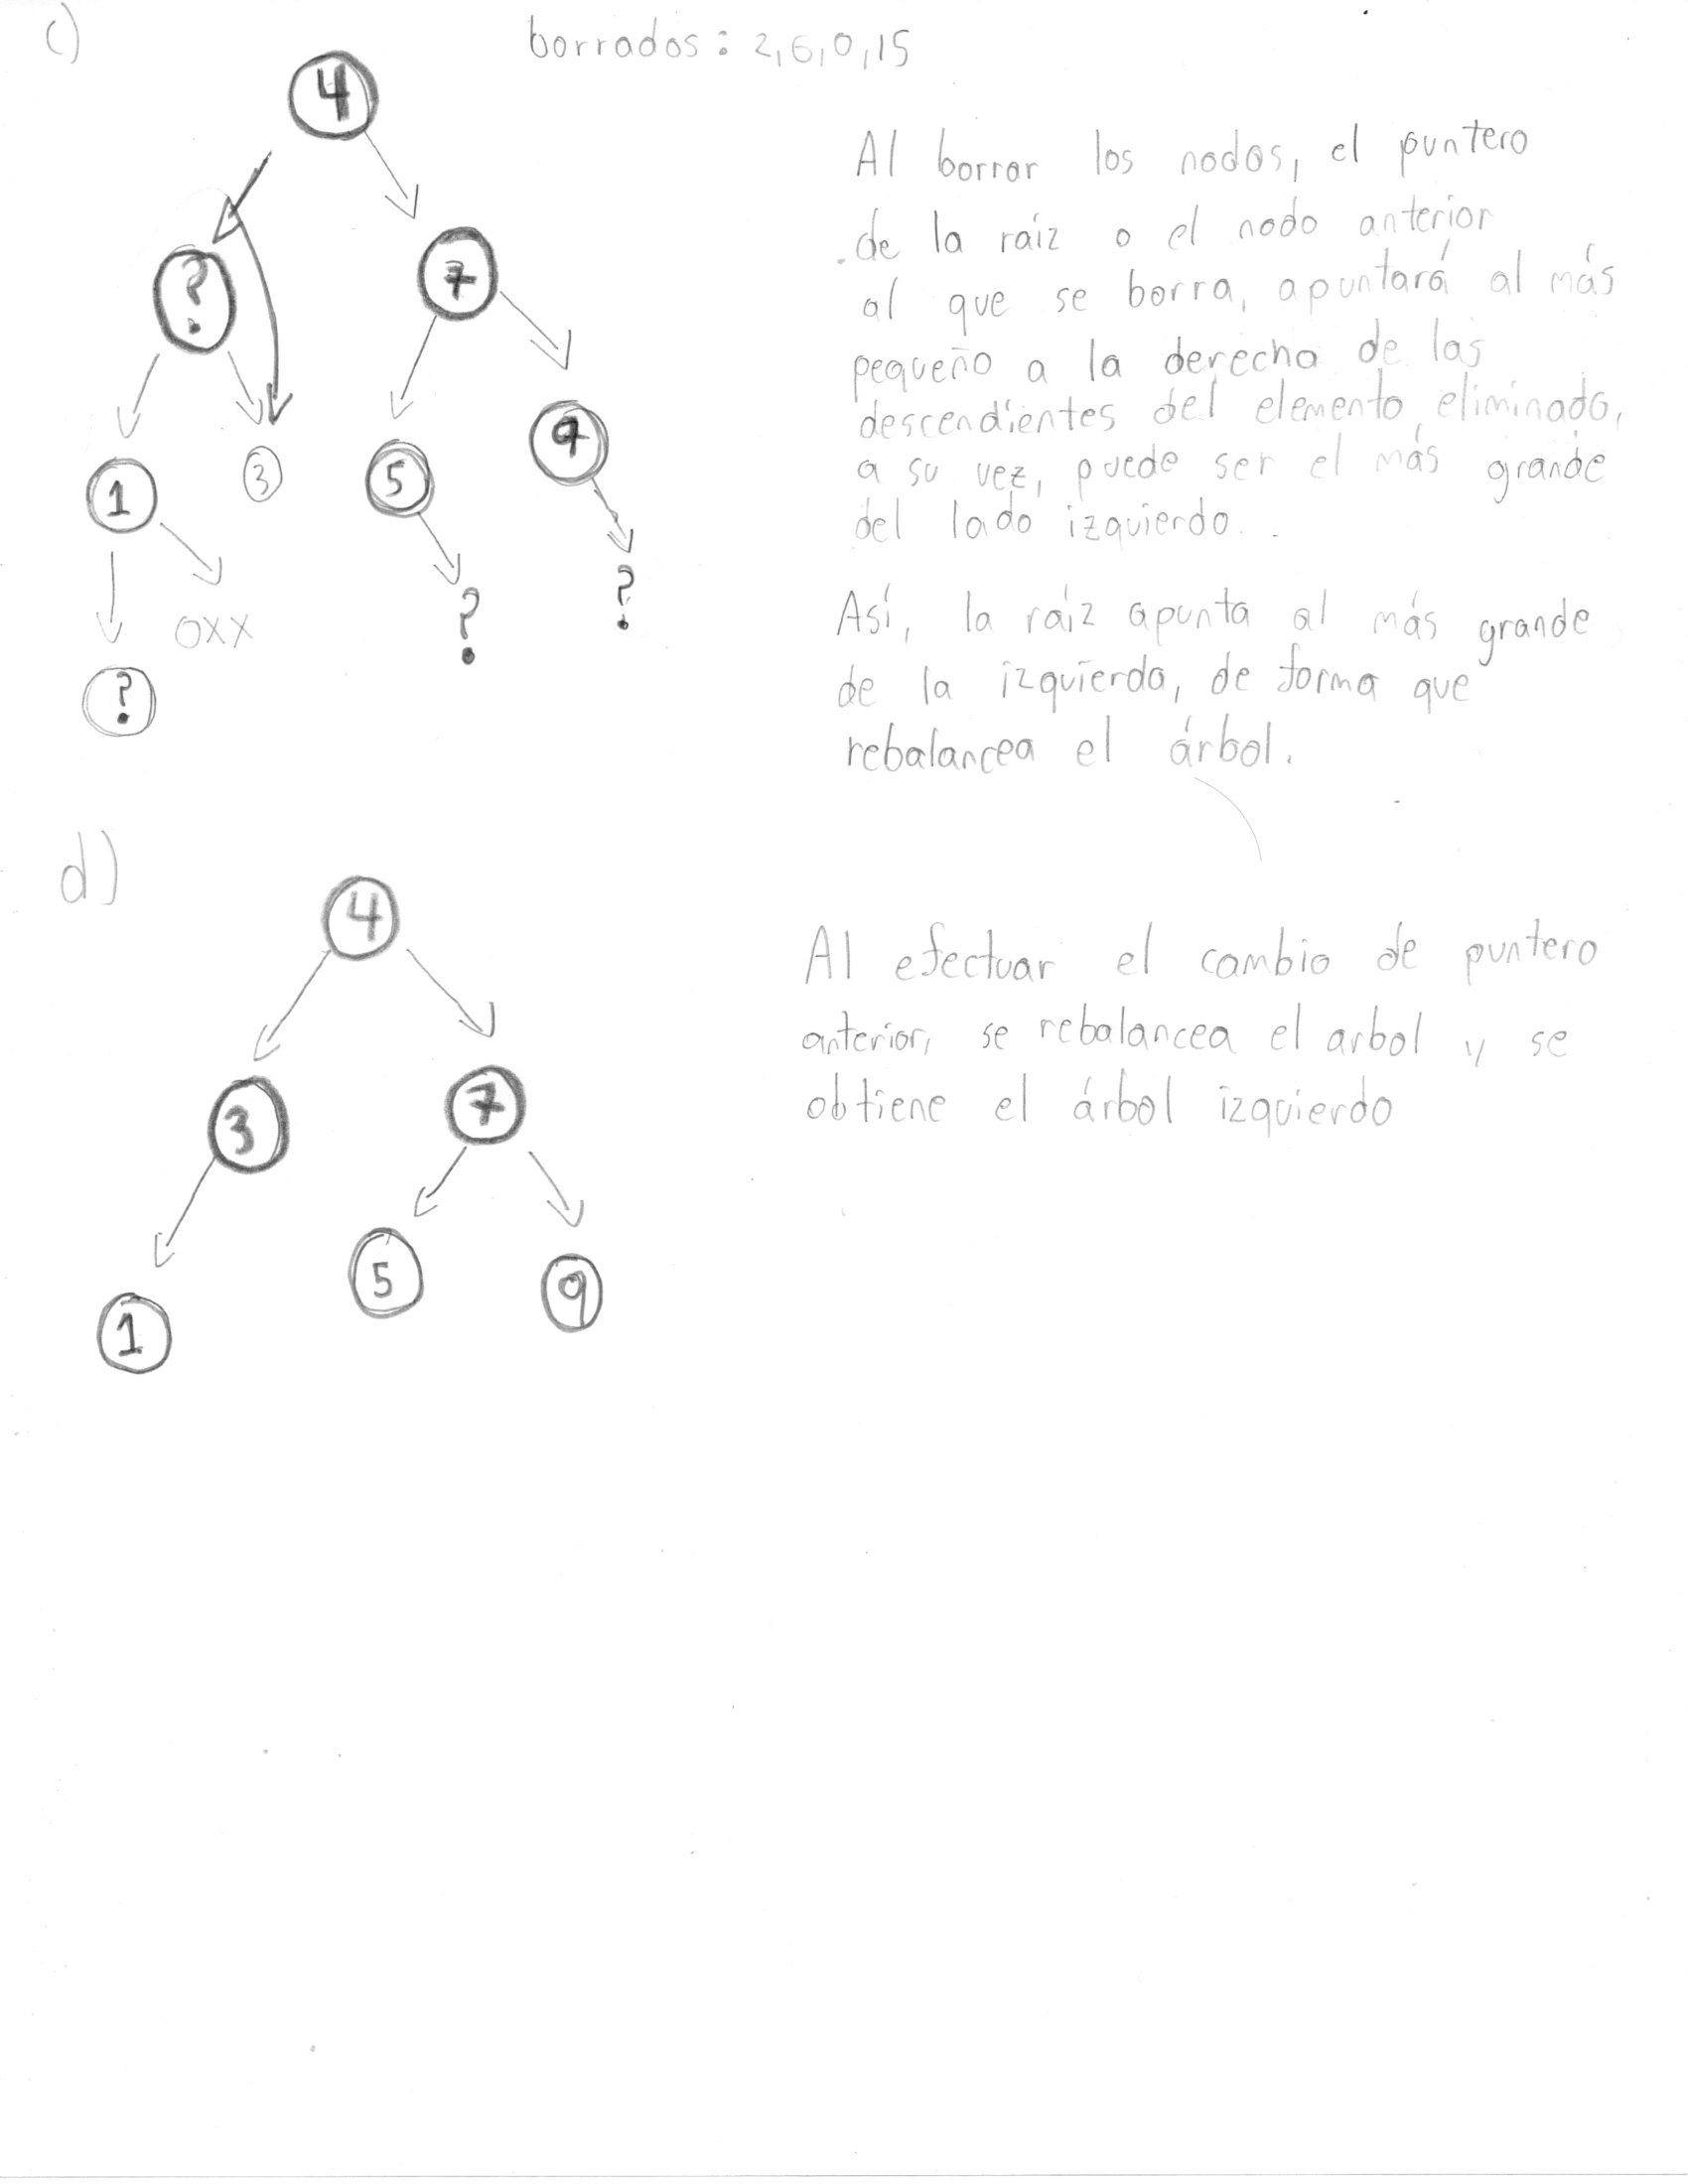
\includegraphics[width=18.5cm]{foto3.jpg}
\centering
\end{figure}
 
\section{Anexos}

\lstinputlisting[language=C++, 
caption=mainBP.cpp
]{mainBP.cpp}

\newpage

\lstinputlisting[language=C++, 
caption=a.cpp
]{a.cpp}

\newpage

\lstinputlisting[language=C++, 
caption=Stack.h
]{Stack.h}

\newpage

\lstinputlisting[language=C++, 
caption=Queue.h
]{Queue.h}
 



\end{document}